% !TEX root = ../thesis.tex

\chapter{Circuit Quantization and Modeling}\label{apx:chp_quantization}

%============================================================
\section{Assigning External Flux Using a Spanning Tree}
%============================================================

A spanning tree supplies a convenient allocation and is the standard tool used to assign external fluxes self-consistently \cite{voolIntroductionQuantumElectromagnetic2017}. In the spanning tree construction, a subgraph is chosen that touches every vertex without closing a loop. The edges left out of the tree are the closure branches, and all external fluxes are assigned to them. In our vector notation, we can order the branches as (tree -- $t$, closure -- $c$). We then define
\begin{align}
    \mathrm{G} = \begin{pmatrix} \mathrm{G}_t & I \end{pmatrix} \quad {\rm and} \quad  \mathrm{B} = \begin{pmatrix} 0 \\ I \end{pmatrix} \, ,
    \label{eq:tree_B}
\end{align}
which solves $\mathrm{G}\mathrm{B}=I$ immediately.
The block $\mathrm{G}_t$ is also fixed.
Expanding $\mathrm{G}\Omega^T = 0$ in the same ordering gives $\mathrm{G}_t\Omega_t^T + \Omega_c^T = 0$, so $\mathrm{G}_t = -\Omega_c^T\left(\Omega_t^{T}\right)^{-1}$, where $\Omega_t$ and $\Omega_c$ are the tree and closure blocks of $\Omega$.
A spanning tree on $N_v$ vertices has $N_v-1$ edges, so $\Omega_t$ is not of full row rank.
For this construction we can simply delete a row.
The cycle space does not depend on the choice, and the resulting $\mathrm{G}$ satisfies $\mathrm{G}\Omega^T = 0$ against the full $\Omega$ as well.
Deleting the root of the tree is the convenient choice and is equivalent to the standard procedure of starting the spanning tree at the ground node.\footnote{Ordering each tree edge by the vertex it feeds, and the vertices so that parents precede children, makes $\Omega_t$ triangular, and its inverse is then triangular with entries in $\{0,\pm1\}$, given by whether an edge lies on the path from the root to a vertex.
The entries of $\mathrm{G}$ thus come out in $\{0,\pm1\}$ as required.}
% A different choice would yield $\mathrm{G}\to M\mathrm{G}$ for invertible $M$, corresponds to a relabeling of loops or a different cycle basis.
% This sends $\Phi_{\rm ext}\to M\Phi_{\rm ext}$ and $\mathrm{B}\to\mathrm{B}M^{-1}$, leaving $\mathrm{B}\Phi_{\rm ext}$ and hence the physics unchanged. 
Typically, the ground node is excluded from the branch analysis at the start, so the root-deletion step is implicit.
Here we have included it explicitly as we treat grounded circuits on equal footing with floating ones. 


%============================================================
\section{Converting Between Physical and Frequency Units for Circuit Parameters}\label{apx:params}
% ============================================================
It is common to work with dimensionless phase $\varphi$ and Cooper-pair number $n$, obtained from the dimensionful node flux $\Phi$ and node charge $Q$ by
\begin{align}
    \varphi = \frac{\Phi}{\phi_0}\,, \quad {\rm and} \quad
    n = \frac{Q}{2e}\, .
    \label{eq:dimless_defs}
\end{align}
Here $e>0$ is the elementary charge of an electron and $\phi_0 = \Phi_0/2\pi = \hbar/2e$ is the reduced flux quantum.
External fluxes and offset charges rescale the same way, with 
\begin{align}
\varphi_{\rm ext} = \frac{\Phi_{\rm ext}}{\phi_0}\, \quad {\rm and} \quad n_g = \frac{Q_g}{2e} \, .
\end{align}
This choice gives the canonical commutator $[\varphi_i, n_j] = i\delta_{ij}$ with no residual $\hbar$.
It also removes $\phi_0$ from the Josephson cosines, so compact directions are $2\pi$-periodic in phase with integer-valued conjugate $n$.

With dimensionless flux and charge operators, circuit parameters are typically quoted as frequencies.
For a single element the charging and inductive energies are related to the physical capacitance $C$ and inductance $L$ by
\begin{align}
 h E_C = \frac{e^2}{2C}, \quad \& \quad
 h E_L = \frac{\phi_0^2}{L}\,,
 \label{eq:EC_EL_scalar}
\end{align}
and the Josephson energy of a junction of critical current $I_c$ by $hE_J = I_c\phi_0$.
Of course, \Cref{eq:EC_EL_scalar} ensures that the energy stored in a capacitor and in an inductor,
\begin{align}
 4 h E_C n^2 = \frac{Q^2}{2C}, \quad \& \quad
 \frac{1}{2} h E_L \varphi^2 = \frac{\Phi^2}{2 L},
\end{align}
is the same in either set of units.
We follow the usual convention of writing $E_J$, $E_C$, $E_L$, and $H$ for the frequencies $E_J/h$, $E_C/h$, $E_L/h$, and $H/h$.

Applying \cref{eq:dimless_defs} to the multimode Hamiltonian defines the frequency-unit matrices
\begin{align}
    \mathcal{E}_C \equiv \frac{e^2}{2h}C^{-1}, \quad
    \mathcal{E}_L \equiv \frac{\phi_0^2}{h}L^*, \quad {\rm and} \quad
    \mathcal{E}_{L_b} \equiv \frac{\phi_0^2}{h}L_b^{-1},
    \label{eq:EC_EL_matrix}
\end{align}
which reduce to \cref{eq:EC_EL_scalar} for a single element.
In these units, \cref{eq:classical_H_full} becomes
\begin{align}
    \mathcal{H}(n,\varphi) = 4\bigl(n-\tilde n_g(t)\bigr)^T\mathcal{E}_C\bigl(n-\tilde n_g(t)\bigr) + \mathcal{U}(\varphi) \, ,
    \label{eq:full_H_dimless}
\end{align}
where the potential energy is
\begin{align*}
    \mathcal{U}(\varphi) &= \frac{1}{2}\varphi^T\mathcal{E}_L\varphi + \varphi^T\tilde\omega_L\mathcal{E}_{L_b}\mathrm{B}_L\varphi_{\rm ext}(t) - \sum_{k\in\mathcal{S}_J}E_{J_k}\cos\bigl([\tilde\omega_J^T\varphi+\mathrm{B}_J\varphi_{\rm ext}(t)]_k\bigr) \, .
\end{align*}
Here $C$ and $L^*$ are the retained $\tilde{C}$ and $\tilde{L}^*$ of the reduced Hamiltonian, so the inverse is taken on the invertible $\tilde{C}$ and never on the singular full node capacitance matrix.
The energy of the system is then given by $h H$.


%============================================================
\section{Product States and Mean-Field Hamiltonians}\label{apx:meanfield}
%============================================================
This appendix gives the construction behind the product-state coordinates of \cref{sec:NumericalSearch}.
This includes the product ansatz and its energy, the mean-field Hamiltonians, the outer optimization over $S$, and the hierarchical diagonalization using the mean-field eigenstates as a basis.
We work through the $\cos(2\varphi)$ KITE of \cref{fig:kite} at each step.

\subsection{The Hamiltonian in a transformed frame}
In the published coordinates $(\varphi,\varphi_\Sigma,\varphi_\Delta)$ of Ref.~\cite{Roverch2026experimental}, with conjugate charges $(n,n_\Sigma,n_\Delta)$, zero offset charge, and the loop phase $\pi+\delta$ shared equally over the four inductors, the KITE Hamiltonian of \cref{fig:kite}(a) is
\begin{align}
    H&=4\,n^T\mathcal E_Cn+E_L\bigl(\varphi_\Sigma^2+\varphi_\Delta^2\bigr)-E_L(\pi+\delta)\,\varphi_\Delta -E_J(1+\epsilon)\cos(\varphi-\varphi_\Sigma+\varphi_\Delta)-E_J(1-\epsilon)\cos(\varphi-\varphi_\Sigma-\varphi_\Delta)\, ,
    \label{eq:kite_H_published}
\end{align}
with the charging matrix
\begin{align*}
    \mathcal E_C=\begin{pmatrix}
        E_{C_S}&E_{C_S}&0\\
        E_{C_S}&E_{C_S}+\dfrac{E_{C_J}}{2(1-\epsilon^2)}&\dfrac{\epsilon E_{C_J}}{2(1-\epsilon^2)}\\
        0&\dfrac{\epsilon E_{C_J}}{2(1-\epsilon^2)}&\dfrac{E_{C_J}}{2(1-\epsilon^2)}
    \end{pmatrix} .
\end{align*}
Here $E_L$ is the inductive energy of each arm, whose two inductors of energy $2E_L$ sit on either side of its junction, and the junction area disorder scales $E_J$ and $C_J$ together by $1\pm\epsilon$.
Each junction spans all three coordinates, while the quadratic coupling is only the $E_{C_S}$ entry between $\varphi$ and $\varphi_\Sigma$ and the $\epsilon E_{C_J}$ entry between $\varphi_\Sigma$ and $\varphi_\Delta$.
We consider static external flux, no voltage sources, and zero offset charge.

Written in the coordinates $\varphi=S\varphi'$ of a transformation $S\in\mathcal A_{\rm relaxed}$, \cref{eq:kite_H_published} becomes
\begin{align}
    H' = 4\,n'^T\mathcal E_C' n' + \tfrac12\varphi'^T\mathcal E_L'\varphi' + b'^T\varphi' - \sum_{k\in\mathcal S_J}E_{J_k}\cos\bigl(\tilde\omega_{J,k}'^T\varphi'+\delta_k\bigr) \, ,
    \label{eq:H_frame}
\end{align}
with $\mathcal E_C'=S^{-1}\mathcal E_C S^{-T}$, $\mathcal E_L'=S^T\mathcal E_L S$, $b'=S^Tb$, and $\tilde\omega_{J,k}'=S^T\tilde\omega_{J,k}$.
Here $b=\tilde\omega_L\mathcal E_{L_b}\B_L\varphi_{\rm ext}$ collects the external flux assigned to the inductors, $\delta_k=[\B_J\varphi_{\rm ext}]_k$ the flux assigned to junction $k$, and $\tilde\omega_{J,k}$ is the $k$th column of $\tilde\omega_J$, so that $\tilde\omega_{J,k}'^T\varphi'$ is the phase across junction $k$.
For the KITE, \cref{eq:kite_H_published} has $\mathcal E_L={\rm diag}(0,2E_L,2E_L)$, $b=(0,0,-E_L(\pi+\delta))$, junction rows $\tilde\omega_{J,1}=(1,-1,1)$ and $\tilde\omega_{J,2}=(1,-1,-1)$, and $\delta_k=0$.
At the parameters of \cref{sec:NumericalSearch}, $E_J=16.83$, $E_{C_J}=4.82$, $E_{C_S}=0.072$, and $E_L=1.27$ GHz with $\epsilon=0.03$ and $\delta=0$, this gives $b=(0,0,-3.99)$ GHz and a charging coupling of $0.072$ GHz.
In the optimized frame of \cref{eq:kite_S_opt} the junction rows become $\tilde\omega_{J,1}'=(1,-1.03,0.13)$ and $\tilde\omega_{J,2}'=(1,0.11,-1.13)$, at the price of off-diagonal quadratic terms,
\begin{align*}
    \mathcal E_C'=\begin{pmatrix}\phantom{-}0.29&-0.55&-0.48\\-0.55&\phantom{-}3.01&-0.46\\-0.48&-0.46&\phantom{-}2.77\end{pmatrix},\quad
    \mathcal E_L'=\begin{pmatrix}0&0&0\\0&2.06&0.38\\0&0.38&2.37\end{pmatrix}
\end{align*}
in GHz, with $b'=(0,2.28,-2.51)$ GHz.

\subsection{Optimization over $S$ with a product state anzatz}

The goal is a transformation $S$ where the products of single-mode states represent the full Hamiltonian well, so that a few eigenstates per mode allow for accurate hierarchical diagonalization.
As a proxy we use the best product approximation to the ground state, as in the optimized coordinates of vibrational structure theory \cite{yagi2012optimized}.
The lower its energy in the full Hamiltonian, the closer the ground state is to a product, and the better a product basis built from the same single-mode states should represent the low-lying levels.
Beginning with a product of normalized single-mode states, $\ket\Psi=\bigotimes_i\ket{\psi_i}$, its energy $E_{\rm prod}=\bra\Psi H'\ket\Psi$ is a variational upper bound on the ground energy $E_0$.
\Cref{fig:meanfield_loops} summarizes the two nested minimizations that follow.

\begin{figure}[t]
    \centering
    % Schematic of the two nested minimizations of Appendix C: the outer BFGS loop over the
% frame S (C.3) wraps the inner self-consistent product-state loop (C.2); the converged
% self-consistent product state exits as the C-normalized optimum S*. Loop labels carry \cref
% references to main.tex equations, so a standalone compile shows them as ??. \input into main.tex via the standalone package.
\documentclass[border=3pt]{standalone}
\usepackage{amsmath,amssymb,braket}
\usepackage{hyperref}
\usepackage[noabbrev]{cleveref}
\usepackage{tikz}
\usetikzlibrary{arrows.meta,positioning,fit,calc}
\newcommand{\costFunc}{\mathcal{F}}
\begin{document}
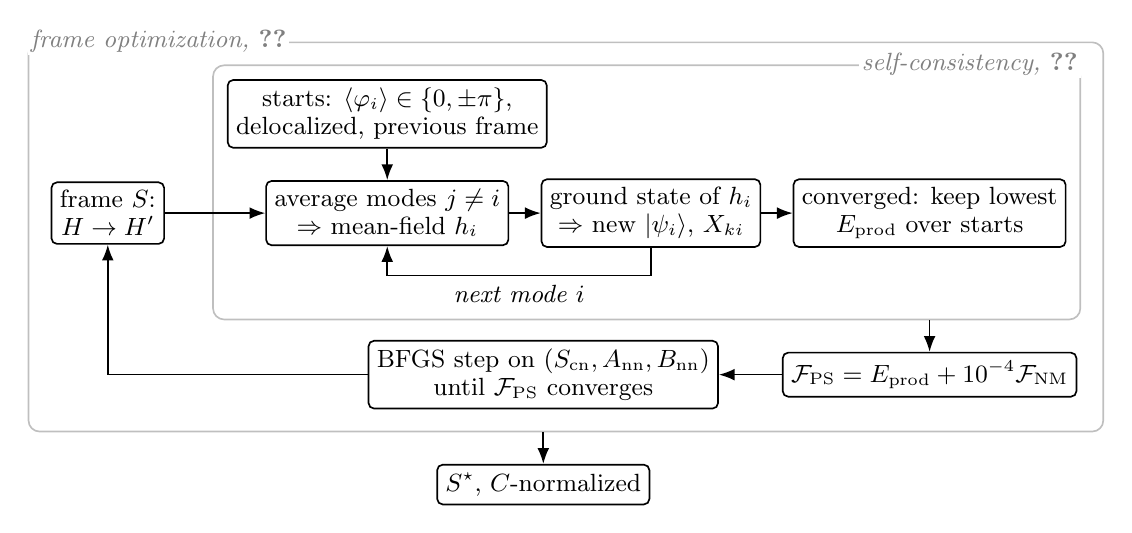
\begin{tikzpicture}[
    font=\small,
    box/.style={draw, rounded corners=2pt, align=center, inner sep=3pt, line width=0.6pt, fill=white},
    loop/.style={draw=gray, draw opacity=0.5, rounded corners=4pt, inner sep=5pt, line width=0.6pt},
    looplab/.style={font=\small\itshape, inner sep=1pt, fill=white, text=gray, text opacity=1, draw opacity=1},
    arr/.style={-{Latex[length=2mm]}, line width=0.6pt},
    lab/.style={font=\small\itshape, inner sep=1pt, fill=white},
    node distance=4mm and 4mm,
]
    % ---- inner loop: starts feed a horizontal ring, converged solutions leave to the right ----
    \node[box] (hi) {average modes $j\neq i$\\[-1pt] $\Rightarrow$ mean-field $h_i$};
    \node[box, right=of hi] (psi) {ground state of $h_i$\\[-1pt] $\Rightarrow$ new $\ket{\psi_i}$, $X_{ki}$};
    \node[box, right=of psi] (keep) {converged: keep lowest\\[-1pt] $E_{\rm prod}$ over starts};
    \node[box, above=of hi] (starts) {starts: $\langle\varphi_i\rangle\in\{0,\pm\pi\}$,\\[-1pt] delocalized, previous frame};
    \draw[arr] (starts) -- (hi);
    \draw[arr] (hi) -- (psi);
    \draw[arr] (psi) -- (keep);
    \coordinate (ret) at ($(psi.south)+(0,-3.5mm)$);
    \draw[arr] (psi.south) -- (ret) -| (hi.south);
    \node[lab, below=0.8mm of {$(ret)!0.5!(ret -| hi.south)$}] (retlab) {next mode $i$};
    \node[loop, fit=(starts)(hi)(psi)(keep)(retlab), label={[looplab, anchor=east]north east:self-consistency, \cref{eq:mean_field_h}}] (inner) {};
    % ---- outer loop: frame on the left, cost and BFGS snaking back below ----
    \node[box, left=6mm of hi.west -| inner.west] (frame) {frame $S$:\\[-1pt] $H\to H'$};
    \draw[arr] (frame) -- (hi);
    \node[box, anchor=north] (cost) at ($(inner.south -| keep.center)+(0,-4mm)$) {$\costFunc_{\rm PS}=E_{\rm prod}+10^{-4}\costFunc_{\rm NM}$};
    \draw[arr] (inner.south -| keep.center) -- (cost);
    \node[box, left=8mm of cost] (bfgs) {BFGS step on $(S_{\rm cn},A_{\rm nn},B_{\rm nn})$\\[-1pt] until $\costFunc_{\rm PS}$ converges};
    \draw[arr] (cost) -- (bfgs);
    \draw[arr] (bfgs.west) -| (frame.south);
    \node[loop, inner sep=8pt, fit=(frame)(inner)(cost)(bfgs), label={[looplab, anchor=west]north west:frame optimization, \cref{eq:H_frame}}] (outer) {};
    % ---- exits ----
    \node[box, anchor=north] (sopt) at ($(outer.south -| bfgs.center)+(0,-4mm)$) {$S^\star$, $C$-normalized};
    \draw[arr] (outer.south -| bfgs.center) -- (sopt);
\end{tikzpicture}
\end{document}

    \caption{{\bf The two nested minimizations of the product-state search.}
    The inner loop converges a product state in a fixed frame: each mode in turn is replaced by the ground state of its mean-field Hamiltonian $h_i$, the full Hamiltonian averaged over the other modes, until $E_{\rm prod}$ stops changing, and the lowest of the solutions reached from the standard starts is kept.
    The outer loop minimizes the cost of \cref{eq:product_cost} over the frame $S$ by BFGS.}
    \label{fig:meanfield_loops}
\end{figure}

Every term of \cref{eq:H_frame} is a product of single-mode operators, so its expectation value in a product state factorizes into single-mode expectation values.
We iteratively minimize each mode's ground state as a function of the single mode eigenstates independently and continue until the overall ground state energy converges.
For diagonalizing each mode, we use a uniform phase grid with eighth-order finite differences, wide enough that the inductive energy at its edge exceeds twice the junction energy the mode sees, fine enough to resolve the zero-point width and the shortest junction wavelength, and enlarged if a converged state reaches its edge.
For the KITE this gives 33 charge states and about 120 grid points per extended mode.

Each step of this iteration diagonalizes a mean-field Hamiltonian, which we denote $h_i$.
This is the full Hamiltonian \cref{eq:H_frame}, with each cosine of a sum of phases expanded by the angle-addition formula, and every operator of a mode other than the one in question replaced by the scalar expectation value of the current product state.
Mode $i$ then sees the average potential the other modes create.
We write the mean-field Hamiltonian $h_i$ in terms of the expectation value  $\langle\quad\rangle$ of the current $\ket{\psi_j}$,
\begin{align}
    h_i&=4\mathcal E'_{C,ii}n_i^2+\tfrac12\mathcal E'_{L,ii}\varphi_i^2
    +\Bigl(b_i'+\sum_{j\neq i}\mathcal E'_{L,ij}\langle\varphi_j\rangle\Bigr)\varphi_i
    +8\sum_{j\neq i}\mathcal E'_{C,ij}\langle n_j\rangle\,n_i \nonumber\\
    &\quad-\sum_kE_{J_k}|z_{ki}|\cos\bigl(\tilde\omega_{J,ki}'\varphi_i+\arg z_{ki}\bigr)\, ,\qquad
    z_{ki}=e^{i\delta_k}\prod_{j\neq i}X_{kj}\, .
    \label{eq:mean_field_h}
\end{align}
Here $X_{kj}=\langle\cos(\tilde\omega'_{J,kj}\varphi_j)\rangle+i\langle\sin(\tilde\omega'_{J,kj}\varphi_j)\rangle$ collects the sine and cosine averages of mode $j$ over one period of junction $k$.
The final $E_{\rm prod}=\bra{\psi_i}h_i\ket{\psi_i}+{\rm const}$.
A mode spread over a full period of a junction has $X_{kj}=0$ and hides that junction from the others, while a mode sharply localized in a junction's well has $|X_{kj}|=1$.
The ground state of $h_i$ is the best choice of $\ket{\psi_i}$ while the other modes are held fixed, so cycling through the modes and updating each in turn ends at a self-consistent set of states, each the ground state of the mean field the others create.

A system can have multiple localized wells, and the converged solution depends on the starting guess.
As a result, we run the iteration from several starts and keep the lowest converged energy.
A start is the set of scalars that builds the first mean-field Hamiltonians.
A displacement start pins every mode at a phase $\varphi_j^{(0)}\in\{0,\pm\pi\}$,
\begin{align}
    \langle n_j\rangle=0\, ,\qquad
    \langle\varphi_j\rangle=\varphi_j^{(0)}\, ,\qquad
    X_{kj}=\cos\bigl(\tilde\omega'_{J,kj}\varphi_j^{(0)}\bigr)+i\sin\bigl(\tilde\omega'_{J,kj}\varphi_j^{(0)}\bigr)\, ,
    \label{eq:start}
\end{align}
which are the expectation values of a state perfectly localized at $\varphi^{(0)}$; the mean phase is only needed for the extended modes, since a compact mode has no inductive terms.
Every junction then enters the first $h_i$ with full amplitude, $|z_{ki}|=1$, and with its cosine shifted by the phase the other modes contribute at $\varphi^{(0)}$, so the iteration relaxes from that classical configuration into the nearest well.
We take all $3^N$ combinations of $0$ and $\pm\pi$.
The delocalized start instead sets $\langle n_j\rangle=\langle\varphi_j\rangle=0$ and every $X_{kj}=0$, so no junction is visible at the first step and each mode begins from the ground state of its quadratic terms alone.
For the KITE, the relevant solutions are the two wells of the $\cos(2\varphi)$ potential, with $\varphi$ near $0$ or $\pi$ and the extended modes displaced to match.
In the published coordinates the wells are degenerate at $E_{\rm prod}=-8.08$ GHz, with $(\varphi,\varphi_\Delta)$ near $(0,0.18)$ or $(\pi,2.96)$, and the delocalized start alone reaches a third solution, a saddle at $+3.83$ GHz with $\langle\varphi_\Delta\rangle=\pi/2$.
In the optimized frame the same starts reach only the two wells, at $-9.43$ GHz.
The ground doublet of the full circuit is the symmetric and antisymmetric combination of the two wells, so a product state localized in one well overlaps each doublet member with weight near one half.
This is why \cref{sec:NumericalSearch} reports the weight outside the doublet, $1-\sum_s|\braket{s|\Psi}|^2$ over the two doublet states, rather than the overlap with the ground state.

The outer optimization minimizes the converged product energy over the frame, with a small tie-break toward the normal-mode cost $\costFunc_{\rm NM}$ of \cref{eq:numerical_normal_cost},
\begin{align}
    \costFunc_{\rm PS}(S)=E_{\rm prod}(S)+10^{-4}\,\costFunc_{\rm NM}(S)\, ,
    \label{eq:product_cost}
\end{align}
minimized over $S\in\mathcal A_{\rm relaxed}$ in the parametrization of \cref{eq:S_numerical} by BFGS with finite-difference gradients, from the identity and from a few random starts.
Each evaluation of $E_{\rm prod}$ runs the mean-field iteration from the standard starts and, as a warm start, from the expectation values of the previous frame.
The discrete block $S_{\rm cc}$ is enumerated separately, and the KITE has one compact mode, so we consider $S_{\rm cc}=\pm1$ and perform a continuous optimization over the six entries of $(S_{\rm cn},A_{\rm nn},B_{\rm nn})$.
We fix the scale afterwards by normalizing each noncompact column to $(S^T\mathcal E_C^{-1}S)_{jj}=1$ in ${\rm GHz}^{-1}$ (i.e., the $C$-normalization of \cref{eq:kite_S_opt}).

\subsection{Hierarchical diagonalization with mean-field leaves}

Hierarchical diagonalization trades the full single-mode grids for a small basis per mode.
For each mode $i$ one keeps $m$ single-mode eigenstates states, which we call leaves, and represent the full Hamiltonian in the $m^N$ products of leaves.
Every single-mode operator $A$ in \cref{eq:H_frame} becomes the $m\times m$ matrix $U_i^\dagger AU_i$, the products of these matrices are assembled into an $m^N\times m^N$ matrix, and its lowest levels are found by dense diagonalization.
The usual leaves are the eigenstates of each mode's own Hamiltonian with the coupling dropped.
For the KITE every junction couples all three modes, so these bare leaves are oscillator and charge states that know nothing of the junctions, and many of them are needed to build a state localized in a junction well.

The mean-field Hamiltonians describe instead what each mode sees in the ground state, so their eigenstates already contain each junction, at the amplitude and phase the other modes give it.
They are a natural single-mode basis for the hierarchical diagonalization of \cref{sec:NumericalSearch}, but they also require more states than a single mean field would.
Each well $w$ has its own $h_i^{(w)}$, and we draw the leaves from both, since the low-lying levels are doublets of the two wells while each mean-field solution describes only one of them.
For each well $w$ and each mode $i$ we take the $m$ lowest eigenvectors of $h_i^{(w)}$ on the single-mode grid.
In the published coordinates the $\varphi_\Sigma$ leaves of the two wells coincide and only the other two modes differ, while in the optimized frame all three differ, with an overlap of $0.37$ between the wells' extended-mode ground states.
We merge the two sets level by level and orthonormalize them by Gram--Schmidt, discarding any vector whose remainder is below $10^{-6}$, until $m$ vectors $U_i$ remain per mode.

In the optimized frame these two-well leaves give a largest error of the four lowest levels of $2\times10^{-3}$ GHz at $m=12$ and $2\times10^{-5}$ GHz at $m=20$.
With leaves from one well only, the second doublet member is poorly represented at small $m$.
Bare leaves, the eigenstates of each mode's own quadratic terms with no mean field, treat both wells alike but see no junction at all, since every junction of the KITE involves all three modes in either frame.
They are an order of magnitude worse than the two-well leaves, at $3\times10^{-2}$ and $5\times10^{-4}$ GHz.

%============================================================
\newpage
\section{Notation}\label{apx:notation}
%============================================================
\Cref{tab:notation} collects the symbols of \cref{sec:Lagrange}, with their dimensions, units, and how they transform with $\trans$.

\begin{table*}[th]
\caption{{\bf Notation of \cref{sec:Lagrange}.}
The circuit has $N$ internal nodes (excluding ground and voltage-source nodes), $N_b$ branches, $N_\ell$ independent loops, and $N_V$ voltage sources.
$N_L$ and $N_J$ count the inductive and Josephson branches, $N_{\rm c}$ the compact coordinates, and $N_d$ the dynamical coordinates.
The last column gives the behavior under $\Phi=Z\tilde\Phi$ if applicable.}
\label{tab:notation}
\scriptsize
\renewcommand{\arraystretch}{1.15}
\begin{tabular*}{\textwidth}{@{\extracolsep{\fill}}llp{0.6\textwidth}l@{}}
\toprule
Symbol & Object $\unitsof{Units}$ & Description & Under $\Phi=Z\tilde\Phi$ \\
\midrule
\multicolumn{4}{@{}l}{\emph{Constants and circuit parameters}}\\
$2e$ & constant &
Cooper-pair charge, with $e>0$ the elementary charge. &
invariant \\
$\Phi_0,\,\phi_0$ & constant $\unitsof{Wb}$ &
Superconducting flux quantum $\Phi_0=h/2e$ and reduced flux quantum $\phi_0=\Phi_0/2\pi$. &
invariant \\
$C_k,\,L_k$ & $\mathbb{R}$ $\unitsof{F}$, $\unitsof{H}$ &
Capacitance and inductance of branch $k$. & invariant \\
$E_{J_k}$ & $\mathbb{R}$ $\unitsof{GHz}$ &
Josephson energy of the junction on branch $k$. Quoted as the frequency $E_{J_k}/h$. &
invariant \\
$\mathcal{S}_L,\,\mathcal{S}_J$ & index sets &
Branches carrying an inductor or a Josephson junction, of sizes $N_L$ and $N_J$. &
invariant \\
\midrule
\multicolumn{4}{@{}l}{\emph{Coordinates and conjugate variables}}\\
$\Phi$ & $\mathbb{R}^{N}$ $\unitsof{Wb}$ &
Node-flux vector, the generalized coordinate of the Lagrangian, with $\Phi_i=\int_{-\infty}^{t}V_i(t')\,dt'$ for the voltage $V_i$ of node $i$ relative to ground. &
$\tilde\Phi=Z^{-1}\Phi$ \\
$\dot\Phi$ & $\mathbb{R}^{N}$ $\unitsof{V}$ &
Node voltages, the generalized velocities. &
$\dot{\tilde\Phi}=Z^{-1}\dot\Phi$ \\
$Q$ & $\mathbb{R}^{N}$ $\unitsof{C}$ &
Node charge conjugate to $\Phi$, with $Q=C\dot\Phi+Q_g$ and $[\Phi_i,Q_j]=i\hbar\delta_{ij}$. &
$\tilde Q=Z^{T}Q$ \\
$\Phi_b$ & $\mathbb{R}^{N_b}$ $\unitsof{Wb}$ &
Branch-flux vector, $\Phi_b=\Omega^T\Phi+\B\Phi_{\rm ext}$.
It is physical rather than a coordinate choice. &
invariant \\
$\Phi_{\rm ext}$ & $\mathbb{R}^{N_\ell}$ $\unitsof{Wb}$ &
External fluxes threading the $N_\ell$ independent loops, including loops broken by capacitors.
Split as $\Phi_{\rm ext}(t)=\Phi_{\rm ext}^{\rm DC}+\Phi_{\rm ext}^{\rm AC}(t)$ into static DC and time-dependent AC parts. &
invariant \\
$V(t)$ & $\mathbb{R}^{N_V}$ $\unitsof{V}$ &
Voltages of the classical source nodes. &
invariant \\
$Q_g$ & $\mathbb{R}^{N}$ $\unitsof{C}$ &
Offset charge, $Q_g=-C_VV(t)+\Omega C_b\B\dot\Phi_{\rm ext}(t)$, entering the Hamiltonian as $Q-Q_g$. &
$\tilde Q_g=Z^{T}Q_g$ \\
$\varphi,\,n$ & $\mathbb{R}^{N}$ &
Dimensionless phase $\varphi=\tilde\Phi/\phi_0$ and Cooper-pair number $n=\tilde Q/2e$. &
as $\Phi$ and $Q$ \\
$\tilde n_g$ & $\mathbb{R}^{N}$ &
Dimensionless offset charge $\tilde n_g=\tilde Q_g/2e$. &
as $Q_g$ \\
$\varphi_{\rm ext}$ & $\mathbb{R}^{N_\ell}$ &
Dimensionless external flux $\varphi_{\rm ext}=\Phi_{\rm ext}/\phi_0$. &
invariant \\
\midrule
\multicolumn{4}{@{}l}{\emph{Circuit matrices}}\\
$\Omega$ & $\{0,\pm1\}^{N\times N_b}$ &
Branch incidence matrix.
Column $k$ has $+1$ at the head node and $-1$ at the tail node of branch $k$, with only the $+1$ for branches to ground or a voltage source. &
$\tilde\Omega^T=\Omega^TZ$ \\
$\omega_L$ & $\{0,\pm1\}^{N\times N_L}$ &
Inductor incidence matrix, the columns of $\Omega$ for $k\in\mathcal{S}_L$. &
$\tilde\omega_L^T=\omega_L^TZ$ \\
$\omega_J$ & $\{0,\pm1\}^{N\times N_J}$ &
Junction incidence matrix, the columns of $\Omega$ for $k\in\mathcal{S}_J$. &
$\tilde\omega_J^T=\omega_J^TZ$ \\
$\G$ & $\{0,\pm1\}^{N_\ell\times N_b}$ &
Loop matrix, whose rows list signed branches around each independent loop, $\G\Omega^T=0$. &
invariant \\
$\G_{JL}$ & rows of $\G$ &
Loops whose branches all carry an inductor or junction, which obey fluxoid quantization $\G_{JL}\Phi_b=\Phi_{\rm ext}$.
The remaining loops are broken by a capacitor and obey Faraday's law. &
invariant \\
$\B$ & $\mathbb{R}^{N_b\times N_\ell}$ &
Flux-assignment matrix distributing the external fluxes over branches, constrained by $\G\B=I$.
The irrotational choice $\Birrot$, with $Z^T\Omega C_b\Birrot=0$, is \cref{eq:irrotational_sol}. &
invariant \\
$\B^{\rm DC}$ & $\mathbb{R}^{N_b\times N_\ell}$ &
Separate assignment of the DC flux $\Phi_{\rm ext}^{\rm DC}$, constrained only by $\G\B^{\rm DC}=I$. &
invariant \\
$\B_L$ & $\mathbb{R}^{N_L\times N_\ell}$ &
Rows of $\B$ for $k\in\mathcal{S}_L$. &
invariant \\
$\B_J$ & $\mathbb{R}^{N_J\times N_\ell}$ &
Rows of $\B$ for $k\in\mathcal{S}_J$. &
invariant \\
$C_b$ & $\mathbb{R}^{N_b\times N_b}$ $\unitsof{F}$ &
Diagonal branch capacitance matrix with entries $C_k$. &
invariant \\
$L_b^{-1}$ & $\mathbb{R}^{N_b\times N_b}$ $\unitsof{H^{-1}}$ &
Diagonal branch inverse-inductance matrix with entries $1/L_k$, and zero on branches without an inductor. &
invariant \\
$C$ & $\mathbb{R}^{N\times N}$ $\unitsof{F}$ &
Node capacitance matrix, $C=\Omega C_b\Omega^T$. &
$\tilde C=Z^{T}CZ$ \\
$L^*$ & $\mathbb{R}^{N\times N}$ $\unitsof{H^{-1}}$ &
Node susceptance matrix, $L^*=\Omega L_b^{-1}\Omega^T$.&
$\tilde L^*=Z^{T}L^*Z$ \\
$C_V$ & $\mathbb{R}^{N\times N_V}$ $\unitsof{F}$ &
Source-coupling matrix, with entry $(i,s)$ the capacitance between node $i$ and source $s$. &
$\tilde C_V=Z^{T}C_V$ \\
$Z$ & $\mathrm{GL}(N,\mathbb{R})$ &
Coordinate transformation, with $\Phi=Z\tilde\Phi$ and $\tilde \Phi = Z^{-1} \Phi$.&
--- \\
\midrule
\multicolumn{4}{@{}l}{\emph{Mode identification and compact coordinates}}\\
$\nullC,\,\nullL,\,\nullJ$ & subspaces of $\mathbb{R}^{N}$ &
Null spaces $\operatorname{null}(C)$, $\operatorname{null}(L^*)$, and $\operatorname{null}(\omega_J^T)$, which define the six mode types of \cref{fig:mode_euler}. &
$Z^{-1}\nullC$, etc. \\
$\mathcal{P}$ & lattice in $\mathbb{R}^{N_{\rm c}}$ &
Periodicity lattice of the compact coordinates, $\mathcal{P}=\{a:\tilde\omega_{J,\rm c}^Ta\in2\pi\mathbb{Z}^{N_J}\}$. &
--- \\
$\mathcal{K}$ & index set &
$N_{\rm c}$ junctions with linearly independent rows of $\tilde\omega_{J,\rm c}^T$. Fixes coordinates in \cref{eq:reference_compact}. &
--- \\
\midrule
\multicolumn{4}{@{}l}{\emph{Frequency units (\cref{apx:params})}}\\
$\mathcal{E}_C$ & $\mathbb{R}^{N_d\times N_d}$ $\unitsof{Hz}$ &
Charging-energy matrix $\mathcal{E}_C=\tfrac{e^2}{2h}\tilde C^{-1}$, giving the charging term $4(n-\tilde n_g)^T\mathcal{E}_C(n-\tilde n_g)$.
Defined on the invertible dynamical block of $\tilde C$. &
$Z^{-1}\mathcal{E}_CZ^{-T}$ \\
$\mathcal{E}_L$ & $\mathbb{R}^{N_d\times N_d}$ $\unitsof{Hz}$ &
Inductive-energy matrix $\mathcal{E}_L=\tfrac{\phi_0^2}{h}\tilde L^*$. &
$Z^{T}\mathcal{E}_LZ$ \\
$\mathcal{E}_{L_b}$ & $\mathbb{R}^{N_b\times N_b}$ $\unitsof{Hz}$ &
Branch inductive-energy matrix $\mathcal{E}_{L_b}=\tfrac{\phi_0^2}{h}L_b^{-1}$. &
invariant \\
\bottomrule
\end{tabular*}
\end{table*}